\documentclass[../lecture-notes-148x210.tex]{subfiles}

\begin{document}

\subsection{Groups}

Throughout the lectures, probably the most important topic is the \textit{group theory}. 

As you can recall from the high school math, typically real-world processes are described using real numbers, denoted by $\mathbb{R}$. For example, to describe the position or the velocity of an object, you would rather use real numbers. 

When it comes to working with computers though, real numbers become very inconvenient to work with. For instance, different programming languages might output different values for quite a straightforward operation \textsf{2.01 + 2.00}. This becomes a huge problem when dealing with cryptography, which must check \textit{precisely} whether two quantities are equal. 
For example, if the person's card number is $N$ and the developed system operates with a different, but very similar card with number $N + k$ for $k \ll N$, then this system can be safely thrown out of the window. See Figure \ref{fig:why_integers}.

\begin{figure}[H]
    \centering
    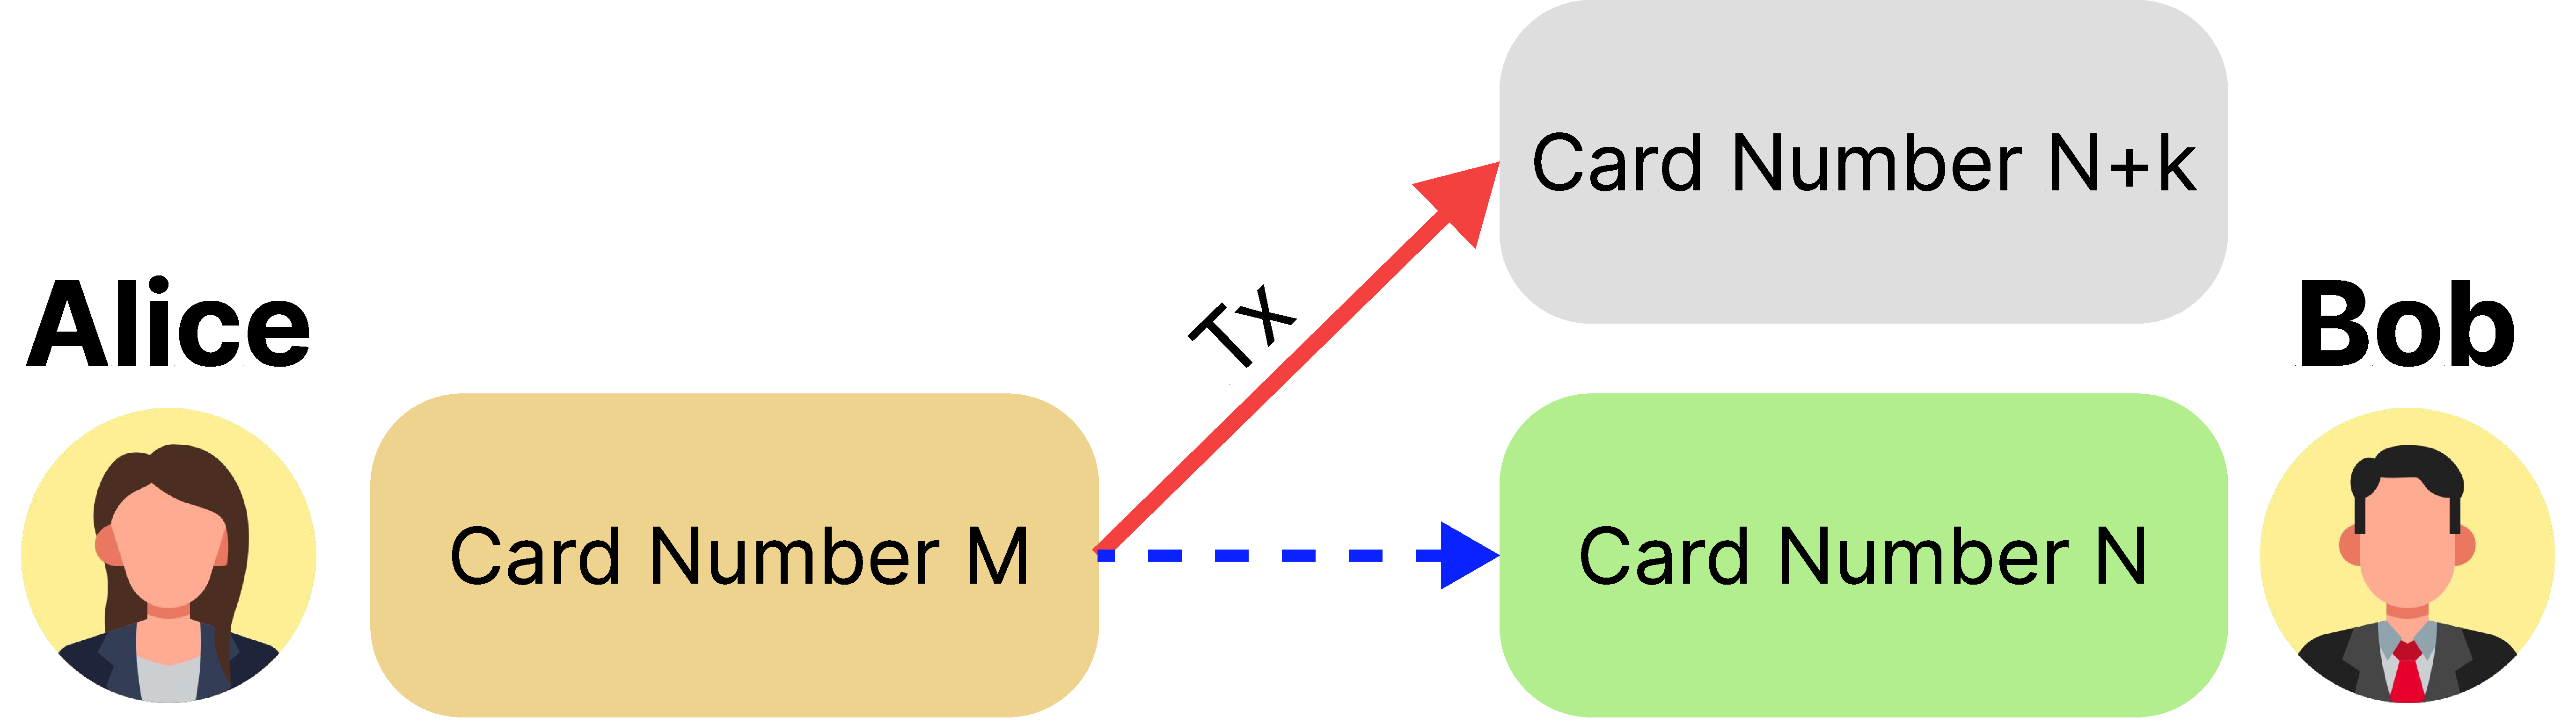
\includegraphics[width=0.8\textwidth]{images/lecture_1/why_integers.pdf}
    \caption{Alice pays to Bob to a card number $N$, but our awesome system pays to $N+k$ instead. Bob would not be happy...}
    \label{fig:why_integers}
\end{figure}

This motivates us to work with integers (denoted by $\mathbb{Z}$), instead. This solves the problem with card numbers, but for cryptography this object is still not really suitable since it is hard to build a secure and reliable protocol exploiting pure integers (without using a more complex structure). 

This motivates us to use a different primitive for dealing with cryptographic systems. Similarly to programmers working with interfaces (or traits, if you are the \textit{Rust} developer), mathematicians also use the so-called \textit{groups} to represent objects obeying a certain set of rules. The beauty is that we do not concretize \textit{how} operations in this set are performed, but rather state the fact that we can somehow combine elements with the pre-defined properties. We can then discover properties of such objects and whenever we apply the concrete ``implementation'' (spoiler, group of points on elliptic curve), these properties would still hold.

\begin{remark}
    Further discussion with abstract objects should be regarded as ``interfaces'' which do not concretize the ``implementation'' of an object. It merely shows the nature of an object without going into the details.
\end{remark}

Now, let us get dirty and define what the \textbf{group} is.

\begin{definition}
    \textbf{Group}, denoted by $(\mathbb{G}, \oplus)$, is a set with a binary operation $\oplus$, obeying the following rules:
    \begin{enumerate}
        \item \textbf{Closure:} Binary operations always outputs an element from $\mathbb{G}$, that is $\forall a,b \in \mathbb{G}: a \oplus b \in \mathbb{G}$.
        \item \textbf{Associativity:} $\forall a,b,c \in \mathbb{G}: (a \oplus b)\oplus c = a \oplus (b \oplus c)$.
        \item \textbf{Identity element:} There exists a so-called identity element $e \in \mathbb{G}$ such that $\forall a \in \mathbb{G}: e \oplus a = a \oplus e = a$.
        \item \textbf{Inverse element:} $\forall a \in \mathbb{G} \; \exists b \in \mathbb{G}: a\oplus b = b \oplus a = e$. We commonly denote the inverse element as $(\ominus a)$.
    \end{enumerate}
\end{definition}

Quite confusing at first glance, right? The best way to grasp this concept is to consider a couple of examples.

\begin{example}
    A group of integers with the regular addition $(\mathbb{Z},+)$ (also called the \textit{additive} group of integers) is a group. Indeed, an identity element is $e_{\mathbb{Z}}=0$, associativity obviously holds, and an inverse for each element $a \in \mathbb{Z}$ is $(\ominus a) := -a \in \mathbb{Z}$. 
\end{example}

\begin{remark}
    We use the term \textbf{additive group} when we mean that the binary operation is addition $+$, while \textbf{multiplicative group} means that we are multiplying two numbers via $\times$\footnote{In this section, regard $\cdot$ and $\times$ as the same operation of multiplication.}.
\end{remark}

\begin{example}
    The multiplicative group of positive real numbers $(\mathbb{R}_{> 0}, \times)$ is a group for similar reasons. An identity element is $e_{\mathbb{R}_{>0}} = 1$, while the inverse for $a \in \mathbb{R}_{>0}$ is defined as $\frac{1}{a}$.
\end{example}

\begin{example}
    The additive set of natural numbers $(\mathbb{N}, +)$ is not a group. Although operation of addition is closed, there is no identity element nor inverse element for, say, $2$ or $10$.
\end{example}

\begin{example}
    That is possible to have the situation when the element $a \in \mathbb{G}$ can be its own inverse, meaning $a = a^{-1}$. This happens when $a^2 = e$. Additionally, we can mention that for any group $\mathbb{G} = \{g, e\}$ with the order $|\mathbb{G}| = 2$ we have $g^2 = e$.
\end{example}

One might ask a reasonable question: suppose you pick $a,b \in \mathbb{G}$. Is $a \oplus b$ the same as $b \oplus a$? Unfortunately, for some groups, this is not true. 

For this reason, it makes sense to give a special name to a group in which the operation is commutative (meaning, we can swap the elements in the operation).

\begin{definition}
    A group $(\mathbb{G},\oplus)$ is called \textbf{abelian} if $\forall a,b \in \mathbb{G}: a \oplus b = b \oplus a$.
\end{definition}

\begin{example}
    The additive group of integers $(\mathbb{Z},+)$ is an abelian group. Indeed, $a + b = b + a$ for any $a,b \in \mathbb{Z}$.
\end{example}

\begin{example}
    The set of $2 \times 2$ matrices with real entries and determinant $1$ (denoted by $\text{SL}(2,\mathbb{R})$) is a group with respect to matrix multiplication. However, this group is not abelian! Take
    \begin{equation*}
        A = \begin{pmatrix}
            1 & 1 \\
            0 & 1
        \end{pmatrix}, \quad B = \begin{pmatrix}
            1 & 0 \\
            1 & 1
        \end{pmatrix}.
    \end{equation*}

    Then, it is easy to verify that
    \begin{equation*}
        AB = \begin{pmatrix}
            2 & 1 \\
            1 & 1
        \end{pmatrix}, \quad BA = \begin{pmatrix}
            1 & 1 \\
            1 & 2
        \end{pmatrix},
    \end{equation*}
    so clearly $AB \neq BA$ -- the elements of $\text{SL}(2, \mathbb{R})$ do not commute.
\end{example}

\begin{remark}
    Further, we will write $ab$ instead of $a \times b$ and $a^{-1}$ instead of $\ominus a$ for the sake of simplicity (and because it is more common in the literature). As mentioned before, it is usually called the \textit{multiplicative notation}.
\end{remark}

Finally, for cryptography it is important to know the number of elements in a group. This number is called the \textit{order} of the group.
\begin{definition}
    The \textbf{order} of a finite group $\mathbb{G}$ is the number of elements in the group. We denote the order of a group as $|\mathbb{G}|$.
\end{definition}
\begin{example}
    Integers modulo $13$, denoted by $\mathbb{Z}_{13}$, is a group with respect to addition modulo $13$ (e.g., $5+12=4$ in $\mathbb{Z}_{13}$). The order of this group is $13$.
\end{example}

Despite the aforementioned definitions, many things are not generally obvious. For example, one might ask whether the identity element is unique. Or, 
whether the inverse element is unique for each group element. For that reason, we formulate the following lemma.

\begin{lemma}
    Suppose $\mathbb{G}$ is a group. Then, the following statements hold:
    \begin{enumerate}
        \item The identity element is unique.
        \item The inverse element is unique for each element: $\forall a \in \mathbb{G} \, \exists! a^{-1} \in \mathbb{G}: aa^{-1} = a^{-1}a = e$.
        \item For all $a,b \in \mathbb{G}$ there is a unique $x \in \mathbb{G}$ such that $ax = b$.
        \item If $ab=ac$ then $b=c$. Similarly, if $xy=zy$ then $x=z$.
    \end{enumerate}
\end{lemma}

Since this guide is not a textbook on abstract algebra, we will not prove all the statements. However, we will prove the first and second one to show the nature of the proofs in abstract algebra.

\textbf{First Statement Proof.} Suppose $e_1,e_2 \in \mathbb{G}$ are both identity elements. Consider $e_1e_2$. From the definition of the identity element, we know that $e_1e_2 = e_1$ and $e_1e_2 = e_2$. Therefore, $e_1 = e_2$.

\textbf{Second Statement Proof.} Take $g \in \mathbb{G}$ and suppose $a,b \in \mathbb{G}$ are both inverses of $g$. By defininition,
\begin{equation*}
    ag = ga = e, \quad bg = gb = e.
\end{equation*}

Now, notice that
\begin{equation*}
    a = ae = a (gb) = (a g) b = e b = b
\end{equation*}

Thus, $a = b$.

\begin{exercise}
    Prove the third and fourth statements.
\end{exercise}

\subsection{Subgroups}

When we are finally comfortable with the concept of a group, we can move on to the concept of a \textit{subgroup}. 

Suppose we have a group $(\mathbb{G},\oplus)$. Suppose one takes the subset $\mathbb{H} \subset \mathbb{G}$. Of course, since all elements in $\mathbb{H}$ are still elements in $\mathbb{G}$, we can conduct operations between them via $\oplus$. 
The natural question to ask is whether $\mathbb{H}$ is a group itself. Yes, but at the same time $\mathbb{H}$ is called a \textbf{subgroup} of $\mathbb{G}$.

\begin{definition}
    A subset $\mathbb{H} \subset \mathbb{G}$ is called a \textbf{subgroup} of $\mathbb{G}$ if $\mathbb{H}$ is a group with respect to the same operation $\oplus$. We denote this as $\mathbb{H} \leq \mathbb{G}$.
\end{definition}

\begin{example}
    Of course, not every subset of $\mathbb{G}$ is a subgroup. Take $(\mathbb{Z}, +)$. If we cut, say, $3$ out of $\mathbb{Z}$ (so we get $\mathbb{H} = \mathbb{Z} \setminus \{3\}$), then $\mathbb{H}$ is not a subgroup of $\mathbb{Z}$ since an element $-3$ does not have an inverse in $\mathbb{H}$. Moreover, it is not closed: take $1,2 \in \mathbb{H}$. In this case, $1+2 = 3 \notin \mathbb{H}$.
\end{example}

\begin{example}
    Now, let us define some valid subgroup of $\mathbb{Z}$. Take $\mathbb{H} = \{3k: k \in \mathbb{Z}\}$ -- a set of integers divisible by $3$ (commonly denoted as $3\mathbb{Z}$). This is a subgroup of $\mathbb{Z}$, since it is closed under addition, has an identity element $0$, and has an inverse for each element $3k$ (namely, $-3k$). That being said, $3\mathbb{Z} \leq \mathbb{Z}$.
\end{example}

These are good examples, but let us consider a more interesting one, which we call a lemma. It is frequently used further when dealing with cosets and normal subgroups, but currently regard this just as an exercise.
\begin{lemma}
    Let $\mathbb{G}$ be a group and $g \in \mathbb{G}$. The centralizer of $g$ is defined to be
    \begin{equation*}
        C_g = \{h \in \mathbb{G}: h g = g h\}
    \end{equation*}

    Then, $C_g$ is a subgroup of $\mathbb{G}$.
\end{lemma}

\begin{exercise}
    Prove the lemma.
\end{exercise}

\subsection{Cyclic Groups}

Probably, cyclic groups are the most interesting groups in the world of cryptography. But before defining them, we need to know how to add/subtract elements multiple times (that is, multiplying by an integer). Suppose 
we have a group $\mathbb{G}$ and $g \in \mathbb{G}$. Then, $g^n$ means multiplying (adding) $g$ to itself $n$ times. If $n$ is negative, then we add $g^{-1}$ to itself $|n|$ times. For $n=0$ we define $g^0 = e$. Now, let us define what the cyclic group is.
\begin{definition}
    Given a group $\mathbb{G}$ and $g \in \mathbb{G}$ the cyclic subgroup generated by $g$ is
    \begin{equation*}
        \langle g \rangle = \{g^n: n \in \mathbb{Z}\} = \{\dots,g^{-3}, g^{-2}, g^{-1}, e, g, g^2, g^3, \dots\}.
    \end{equation*}
\end{definition}

\begin{example}
    Consider the group of integers modulo $12$, denoted by $\mathbb{Z}_{12}$. Consider $2 \in \mathbb{Z}_{12}$, the group generated by $2$ is then
    \begin{equation*}
        \langle 2 \rangle = \{2,4,6,8,10, 0\}
    \end{equation*}
\end{example}

\begin{definition}
    We say that a group $\mathbb{G}$ is \textbf{cyclic} if there exists an element $g \in \mathbb{G}$ such that $\mathbb{G}$ is generated by $g$, that is, $\mathbb{G} = \langle g \rangle$.
\end{definition}

\begin{example}
    The group of integers $(\mathbb{Z},+)$ is an infinite cyclic group. Indeed, it is generated by $1$.
\end{example}

\subsection{Isomorphisms and Endomorphisms}

Finally, we will define the concept of isomorphisms and endomorphisms. These are important concepts in the world of cryptography, since they allow us to compare different groups. Namely, 
suppose we have two groups $(\mathbb{G},\oplus)$ and $(\mathbb{H}, \odot)$. Is there any way to state that these two groups are the same? The answer is yes, and this is done via isomorphisms.

\begin{definition}
    A function $\varphi: \mathbb{G} \to \mathbb{H}$ is called an \textbf{homomorphism} if it is a function that preserves the group operation, that is, 
    \begin{equation*}
        \forall a,b \in \mathbb{G}: \varphi(a \oplus b) = \varphi(a) \odot \varphi(b).
    \end{equation*}
\end{definition}

\begin{definition}
    An \textbf{isomorphism} is a bijective homomorphism.
\end{definition}

\begin{definition}
    If there exists an isomorphism between two groups $\mathbb{G}$ and $\mathbb{H}$, we say that these groups are isomorphic and write $\mathbb{G} \cong \mathbb{H}$.
\end{definition}

\begin{example}
    Consider the group of integers $(\mathbb{Z},+)$ and the group of integers modulo $12$ $(\mathbb{Z}_{12},+)$. The function $\varphi: \mathbb{Z} \to \mathbb{Z}_{12}$ defined as $\varphi(x) = x \;\text{mod}\; 12$ is a homomorphism. Indeed:
    \begin{equation*}
        \varphi(a+b) = (a+b) \;\text{mod}\; 12 = (a \;\text{mod}\; 12) + (b \;\text{mod}\; 12) = \varphi(a) + \varphi(b).
    \end{equation*}

    However, this function is not an isomorphism, since it is not bijective. For example, $\varphi(0) = \varphi(12) = 0$.
\end{example}

\begin{example}
    Additive group of reals $(\mathbb{R}, +)$ and the multiplicative group of positive reals $(\mathbb{R}_{>0}, \times)$ are isomorphic. The function $\varphi: \mathbb{R} \to \mathbb{R}_{>0}$ defined as $\varphi(x) = e^x$ is an isomorphism. Indeed:
    \begin{equation*}
        \varphi(a+b) = e^{a+b} = e^a \cdot e^b = \varphi(a) \cdot \varphi(b).
    \end{equation*}
    Thus, $\varphi$ is a homomorphism. It is also injective since $e^x = e^y \implies x=y$. Finally, it is obviously onto. This means $(\mathbb{R}, +) \cong (\mathbb{R}_{>0}, \times)$.
\end{example}

\begin{example}
    All groups of order $2$ are isomorphic to $\mathbb{Z}_2$. Indeed, let $\mathbb{G} = \{g,e\}$ -- any group of order 2, and define $\varphi: \mathbb{Z}_2 \to \mathbb{G}$ as $\varphi(0) = e$ and $\varphi(1) = g$. This is an isomorphism.
\end{example}

A generalization of the above example is the following quite interesting theorem:

\begin{theorem}
    Suppose $\mathbb{G} = \langle g \rangle$ is a finite cyclic group, meaning $|G| = n \in \mathbb{N}$. Then, $\mathbb{G} \cong \mathbb{Z}_n$.
\end{theorem}

\textbf{Idea of the proof.} Define a function $\varphi: \mathbb{Z}_n \to \mathbb{G}$ as $m \mapsto g^m$. One can prove that this is an isomorphism.

Here, it is quite evident that isomorphism tells us that the groups have the same structure. Moreover, it is correct to say that if $\mathbb{G} \equiv \mathbb{H}$, then $\mathbb{G}$ and $\mathbb{H}$ are \textit{equivalent} since $\cong$ is an equivalence relation.

\textbf{Exercise (*).} Prove that $\cong$ is an equivalence relation.

Finally, we will define the concept of an endomorphism and automorphism to finish the section.

\begin{definition}
    An \textbf{endomorphism} is a function $\varphi$ which maps set $X$ to itself ($\varphi: X \to X$).
\end{definition}

\begin{definition}
    An \textbf{automorphism} is an isomorphic endomorphism.
\end{definition}

\begin{example}
    Given a group $\mathbb{G}$, fixate $a \in \mathbb{G}$. The map $\varphi: x \mapsto axa^{-1}$ is an automorphism.
\end{example}

Last two definitions are especially frequently used in Elliptic Curves theory.

\subsection{Fields}

Although typically one introduces rings before fields, we believe that for the basic understanding, it is better to start with fields. 

Notice that when dealing with groups, we had a single operation $\oplus$, which, depending on the context, is either interpreted as addition or multiplication. 
However, fields allow to extend this concept a little bit further by introducing a new operation, say, $\odot$, which, combined with $\oplus$, allows us to perform the basic arithmetic.

This is very similar to the real or rational numbers, for example. We can add, subtract, multiply, and divide them. This is exactly what fields are about, but in a more abstract way. That being said, let us see the definition.

\begin{definition}
    A \textbf{field} is a set $\mathbb{F}$ with two operations $\oplus$ and $\odot$ such that:
    \begin{enumerate}
        \item $(\mathbb{F}, \oplus)$ is an abelian group with identity $e_{\oplus}$.
        \item $(\mathbb{F} \setminus \{e_{\oplus}\}, \odot)$ is an abelian group.
        \item The \textbf{distributive law} holds: $\forall a,b,c \in \mathbb{F}: a \odot (b \oplus c) = (a \odot b) \oplus (a \odot c)$.
    \end{enumerate}
\end{definition}

What this definition basically states is that we can perform the following operations:
\begin{enumerate}
    \item Addition: $a \oplus b$, inherited from group structure $(\mathbb{F}, \oplus)$.
    \item Subtraction: $a \oplus (\ominus b)$, inherited from group structure $(\mathbb{F}, \oplus)$.
    \item Multiplication: $a \odot b$, inherited from group structure $(\mathbb{F} \setminus \{e_{\oplus}\}, \odot)$.
    \item Division: $a \odot b^{-1}$, except for $b=0$, inherited from group structure $(\mathbb{F} \setminus \{e_{\oplus}\}, \odot)$.
\end{enumerate}

\begin{example}
    The set of real numbers $(\mathbb{R}, +, \times)$ is obviously a field.
\end{example}

\begin{example}
    The set of complex numbers $(\mathbb{C}, +, \times)$ is also a field. Indeed, let us see how we can perform operations. Suppose we are given $z = a_0 + a_1i$ and $w = b_0 + b_1i$ with $i^2+1=0$. In this case:
    \begin{enumerate}
        \item Addition: $z + w = (a_0 + b_0) + (a_1 + b_1)i$.
        \item Subtraction: $z - w = (a_0 - b_0) + (a_1 - b_1)i$.
        \item Multiplication: $z \cdot w = (a_0b_0 - a_1b_1) + (a_0b_1 + a_1b_0)i$.
        \item Division: $z / w = \frac{a_0b_0 + a_1b_1}{b_0^2 + b_1^2} + \frac{a_1b_0 - a_0b_1}{b_0^2 + b_1^2}i$.
    \end{enumerate}
\end{example}

Interestingly though, it is very difficult to come up with some more complicated, non-trivial examples. For that reason, we will simply move to the most central field used in cryptography -- finite fields.

\subsection{Finite Fields}
Recall: we do not like reals, we want to operate with integers! But notice that $(\mathbb{Z},+,\times)$ does not form a field since division is not closed. For that reason, fixate some integer $p$ and consider the set $\mathbb{Z}_p := \{0,1,2,\dots,p-2,p-1\}$. Now, we will define operations as follows:

\textbf{Addition.} To add $a,b \in \mathbb{Z}_p$, add them as usual to get $c \gets a+b$. However, this way, operation is not closed, since $c$ might be easily greater than $p-1$ (e.g., for $a=b=p-2$). To fix this, take $c' \in \mathbb{Z}_p$ such that $c \equiv c' \pmod{p}$ (or, written more concisely, $c' = (a+b) \;\text{mod} \; p$). 

\begin{example}
    Take $p=5$. Then, $3+4 = 2$ in $\mathbb{Z}_5$ since $c=3+4=7$ and $7 \equiv 2 = c' \pmod{5}$.
\end{example}

\textbf{Multiplication and subtraction.} The algorithm is the same. Find $c \gets ab$ or $c \gets a-b$, respectively, and find $c' \in \mathbb{Z}_p$ such that $c' \equiv c \pmod{p}$.

\begin{example}
    Again, suppose $p=5$. Then, $3 \cdot 4 = 2$ in $\mathbb{F}_5$ since $c=3 \cdot 4 = 12$ and $12 \equiv 2 = c' \pmod{5}$. Similarly, $3-4 = 4$ in $\mathbb{F}_5$ since $c=3-4=-1$ and $-1 \equiv 4 = c' \pmod{5}$.
\end{example}

\textbf{Inversion.} Inversion is a bit more tricky. Recall that $(\mathbb{Z}_p \setminus \{0\}, \times)$ must be an abelian group, meaning that for each $a \in \mathbb{Z}_p$ there should be some $x \in \mathbb{Z}_p$ such that $ax = 1$ (multiplication in a sense of definition above). In other words, we need to solve the modular equation:
\begin{equation*}
    ax \equiv 1 \pmod{p}.
\end{equation*}

Note that there is no guarantee that for any $a \in \mathbb{Z}_p \setminus \{0\}$ we might find such $x$. For example, take $p=10$ and $a=2$. Then, $2x \equiv 1 \pmod{10}$ has no solution. 

The only way to guarantee that for any $a \in \mathbb{Z}_p \setminus \{0\}$ we might find such $x$ is to take $p$ to be a prime number. This is the reason why we call such fields \textbf{prime fields} (or, in many cases, one calls them \textbf{finite fields}).

So finally, with all the definitions, we can define the finite field.

\begin{definition}
    A \textbf{finite field} (or \textit{prime field}) is a set with prime number $p$ of elements $\{0,1,\dots,p-2,p-1\}$, in which operations are defined ``modulo $p$'' (see details above). 

    Typically, finite fields are denoted as $\mathbb{F}_p$ or $\text{GF}(p)$.
\end{definition}

Finite fields is the core object in cryptography. Instead of real numbers or pure integers, we will almost always use finite fields.

\begin{remark}
    In many cases, one might encounter both $\mathbb{F}_p$ and $\mathbb{Z}_p$ notations. The difference is the following: when one refers to $\mathbb{Z}_p$, it is typically assumed that the operations are performed in the ring\footnote{We have not defined as of now what ring is, but, roughly speaking, this is a field without multiplicative inverses} of integers modulo $p$ (meaning, we need only addition, subtraction, and multiplication in the protocol), while division is of little interest. When one refers to $\mathbb{F}_p$, it is typically assumed that we need full arithmetic (including division) for the procool.
\end{remark}

\begin{example}
    Consider $9, 14 \in \mathbb{F}_{17}$. Some examples of calculations:
    \begin{enumerate}
        \item $9+14 = 6$.
        \item $9-14 = 12$.
        \item $9 \times 14 = 7$.
        \item $14^{-1} = 11$ since $14 \cdot 11 = 154 \equiv 1 \pmod{17}$.
    \end{enumerate}
\end{example}

\subsection{Some Fun: Group Implementation in Rust}

In programming, we can think of a group as an interface, having a single binary operation defined, that obeys the rules of closure, associativity, identity element, and inverse element.

For that reason, we might even code a group in Rust! We will also write a simple test to check whether the group is valid and whether the group is abelian.

\textbf{Trait for Group.} First, we define a trait for a group. We will define a group as a trait with the following methods:
\begin{lstlisting}[language=Rust]
/// Trait that represents a group.
pub trait Group: Sized {
    /// Checks whether the two elements are equal.
    fn eq(&self, other: &Self) -> bool;
    /// Returns the identity element of the group.
    fn identity() -> Self;
    /// Adds two elements of the group.
    fn add(&self, a: &Self) -> Self;
    /// Returns the negative of the element.
    fn negate(&self) -> Self;
    /// Subtracts two elements of the group.
    fn sub(&self, a: &Self) -> Self {
        self.add(&a.negate())
    }
}
\end{lstlisting}

\textbf{Checking group validity.} Now observer the following: we get closure for free, since the compiler will check whether the return type of the operation is the same as the type of the group. 
However, there is no guarantee that associativity holds, and our identity element is at all valid. For that reason, we need to somehow additionally check the
validity of implementation.

We propose to do the following: we will randomly sample three elements from the group $a,b,c \xleftarrow[]{R} \mathbb{G}$ and check our three properties:
\begin{enumerate}
    \item $a \oplus (b \oplus c) \xlongequal{?} (a \oplus b) \oplus c$.
    \item $a \oplus e \xlongequal{?} e \oplus a \xlongequal{?} a $.
    \item $a \oplus (\ominus a) \xlongequal{?} (\ominus a) \oplus a \xlongequal{?} e$.
\end{enumerate}

Additionally, if we want to verify whether the group is abelian, we can check whether $a \oplus b \xlongequal{?} b \oplus a$. 

For that reason, for the check, we require the group to be samplable (i.e. we can randomly sample elements from the group):
\begin{lstlisting}[language=Rust]
/// Trait for sampling a random element from a group.
pub trait Samplable {
    /// Returns a random element from the group.
    fn sample() -> Self;
}
\end{lstlisting}

And now, our test looks as follows:
\begin{lstlisting}[language=Rust]
/// Number of tests to check the group properties.
const TESTS_NUMBER: usize = 100;

/// Asserts that the given group G is valid.
/// A group is valid if the following properties hold:
/// 1. Associativity: (a + b) + c = a + (b + c)
/// 2. Identity: a + e = a = e + a
/// 3. Inverse: a + (-a) = e = (-a) + a
pub fn assert_group_valid<G>()
where
    G: Group + Samplable,
{
    for _ in 0..TESTS_NUMBER {
        // Take random three elements
        let a = G::sample();
        let b = G::sample();
        let c = G::sample();

        // Check whether associativity holds
        let ab_c = a.add(&b).add(&c);
        let a_bc = a.add(&b.add(&c));
        let associativity_holds = ab_c.eq(&a_bc);
        assert!(associativity_holds, "Associativity does not hold for the given group");

        // Check whether identity element is valid
        let e = G::identity();
        let ae = a.add(&e);
        let ea = e.add(&a);
        let identity_holds = ae.eq(&a) && ea.eq(&a);
        assert!(identity_holds, "Identity element does not hold for the given group");

        // Check whether inverse element is valid
        let a_neg = a.negate();
        let a_neg_add_a = a_neg.add(&a);
        let a_add_a_neg = a.add(&a_neg);
        let inverse_holds = a_neg_add_a.eq(&e) && a_add_a_neg.eq(&e);
        assert!(inverse_holds, "Inverse element does not hold for the given group");
    }
}

/// Asserts that the given group G is abelian.
/// A group is an abelian group if the following property holds:
/// a + b = b + a for all a, b in G (commutativity)
pub fn assert_group_abelian<G>()
where
    G: Group + Samplable,
{
    for _ in 0..TESTS_NUMBER {
        assert_group_valid::<G>();

        // Take two random elements
        let a = G::sample();
        let b = G::sample();

        // Check whether commutativity holds
        let ab = a.add(&b);
        let ba = b.add(&a);
        assert!(ab.eq(&ba), "Commutativity does not hold for the given group");
    }
}    
\end{lstlisting}

\textbf{Testing the group $(\mathbb{Z}, +)$.} And now, we can define a group for integers and check whether it is valid and abelian:
\begin{lstlisting}[language=Rust]
use crate::group::{Group, Samplable};
use rand::Rng;

/// Implementing group for Rotation3<f32>
impl Group for i64 {
    fn eq(&self, other: &Self) -> bool {
        self == other
    }

    fn identity() -> Self {
        0i64
    }

    fn add(&self, a: &Self) -> Self {
        self + a
    }

    fn negate(&self) -> Self {
        -self
    }
}

impl Samplable for i64 {
    fn sample() -> Self {
        let mut gen = rand::thread_rng();

        // To prevent overflow, we choose a smaller range for i64
        let min = i64::MIN / 3; 
        let max = i64::MAX / 3;
        gen.gen_range(min..max)
    }
}
\end{lstlisting}

Just a small note: since we cannot generate infinite integers, we restrict the range of integers to prevent overflow. So, 
for the sake of simplicity, we divide the range of integers by $3$, in which overflow never occurs.

And now, the moment of truth! Let us define some tests and run them:
\begin{lstlisting}[language=Rust]
#[cfg(test)]
mod tests {
    use super::*;
    use group::*;

    #[test]
    fn test_integers_are_group() {
        assert_group_valid::<i64>()
    }

    #[test]
    fn test_integers_are_abelian() {
        assert_group_abelian::<i64>();
    }
}
\end{lstlisting}

Both tests pass! Now let us consider something a bit trickier.

\textbf{Testing the group $\text{SO}(3)$.} We can define a group for $3 \times 3$ rotation matrices. Of course, composition of two rotation is not commutative, so we expect the abelian test to fail. However,
the group is still valid! For example, there is an identity rotation matrix $E$, and for each rotation matrix $A \in \text{SO}(3)$, there exists a rotation matrix $A^{-1} \in \text{SO}(3)$ such that $AA^{-1} = A^{-1}A = E$. Finally,
the associativity holds as well.

We will use the \texttt{nalgebra} library for this purpose, which contains the implementation of rotation matrices. So our implementation can look as follows:
\begin{lstlisting}[language=Rust]
/// A threshold below which two floating point numbers are considered equal.
const EPSILON: f32 = 1e-6;

/// Implementing group for Rotation3<f32>
impl Group for Rotation3<f32> {
    fn eq(&self, other: &Self) -> bool {
        // Checking whether the norm of a difference is small
        let difference = self.matrix() - other.matrix();
        difference.norm_squared() < EPSILON
    }

    fn identity() -> Self {
        Rotation3::identity()
    }

    fn add(&self, a: &Self) -> Self {
        self * a
    }

    fn negate(&self) -> Self {
        self.inverse()
    }
}

impl Samplable for Rotation3<f32> {
    fn sample() -> Self {
        let mut gen = rand::thread_rng();

        // Pick three random angles
        let roll = gen.gen_range(0.0..1.0);
        let pitch = gen.gen_range(0.0..1.0);
        let yaw = gen.gen_range(0.0..1.0);

        Rotation3::from_euler_angles(roll, pitch, yaw)
    }
}
\end{lstlisting}

Here, there are two tricky moments:
\begin{enumerate}
    \item We cannot compare floating point numbers directly, since they might differ by a small amount. For that reason, we define a small threshold $\varepsilon$. We say that two matrices are equal iff the norm\footnote{one can think of norm as being the measure of ``distance'' between two objects. Similarly, we can define norm not only on matrices, but on vectors as well.} of their difference is less than $\varepsilon$.
    \item To generate a random rotation matrix, we generate three random angles and create a rotation matrix from these angles.
\end{enumerate}

\subsection{Exercises}

\end{document}
